\section*{Step 1}

\begin{custombox}[label={box:Q1}]{Step 1}
	Review the Jupyter Notebook \verb|E3.ipynb| and:
	\begin{enumerate}[label=(\alph*)]
		\item Create a summary of the code therein.
		\item Are there any learnings from this code that you wish to highlight?
	\end{enumerate}
\end{custombox}

\vspace{5mm}

This Python Notebook \verb|E3.ipynb| presents an analysis of various regression models applied to a dataset using polynomial features of different degrees. The models analyzed include Linear Regression, Support Vector Machine (SVM) Regression, Random Forest, Gradient Boosting, K-Nearest Neighbors (KNN), and Neural Networks. The performance of each model is evaluated based on metrics such as R-squared, Mean Squared Error (MSE), Durbin-Watson, and Jarque-Bera statistics. \\

We use the dataset given in \verb|E3-MLR3.xlsx|. The dataset contains $548$ samples of $(y, x_1)$ to train the model and $152$ samples of $(y, x_1)$ to test the model. 

\begin{figure}[H]
	\centering
	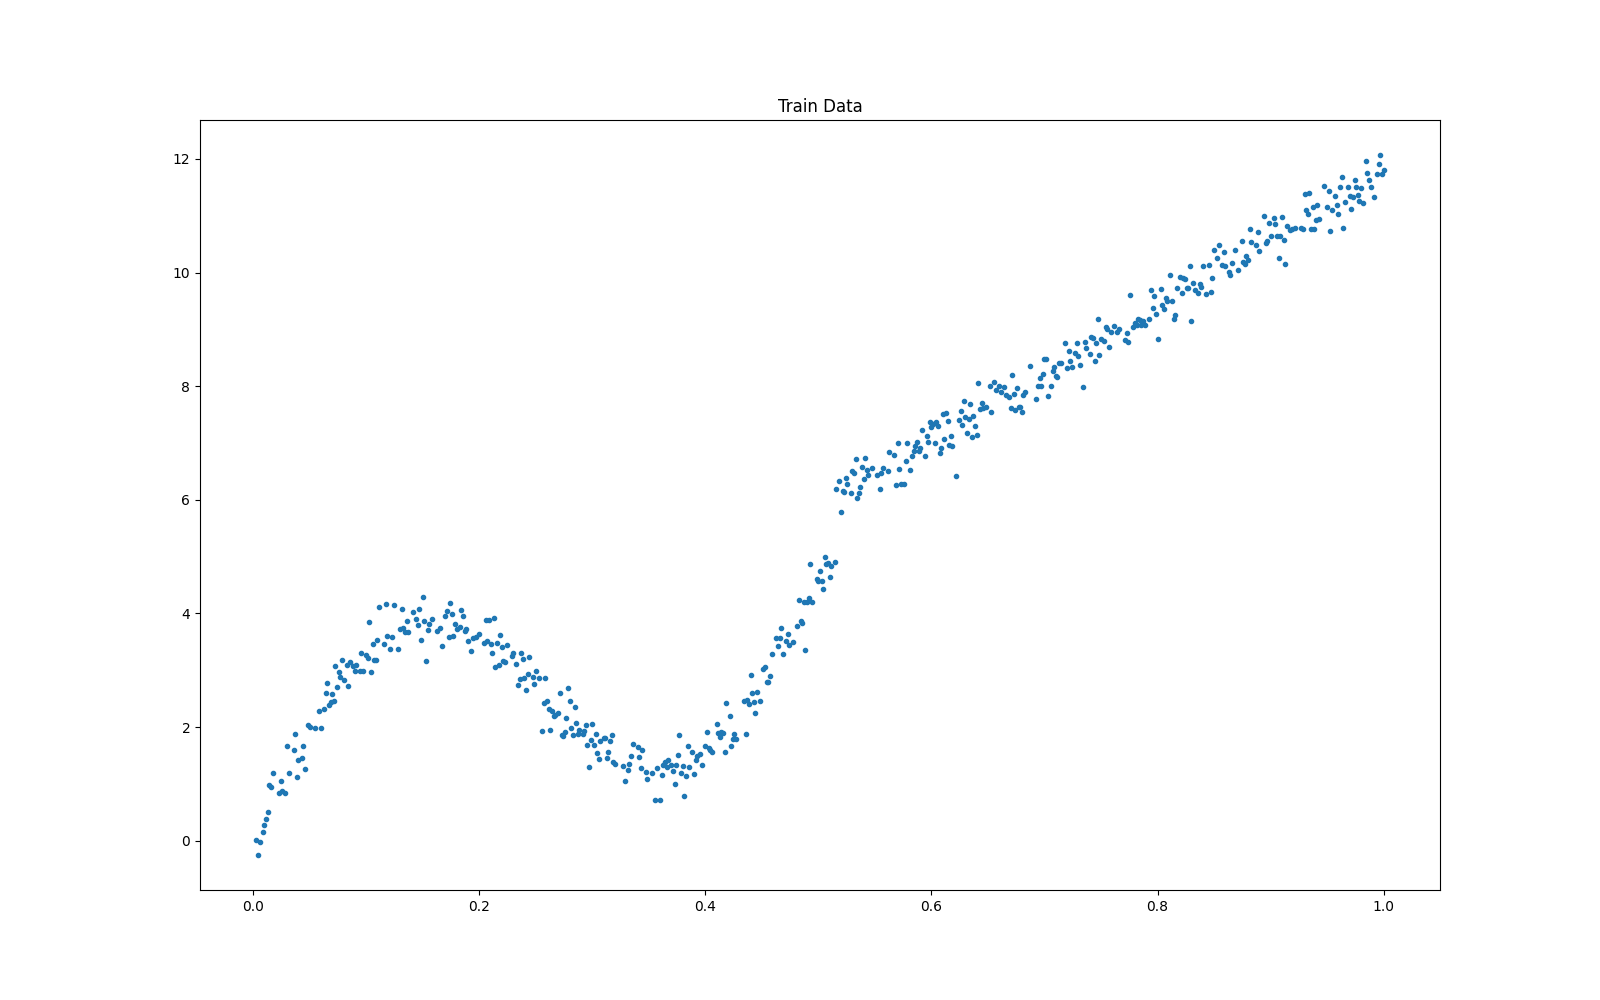
\includegraphics[width=0.7\linewidth]{./Images/E3-MLR3-Train.png}
	\caption{Training Data used in the analysis}
\end{figure}

\begin{figure}[H]
	\centering
	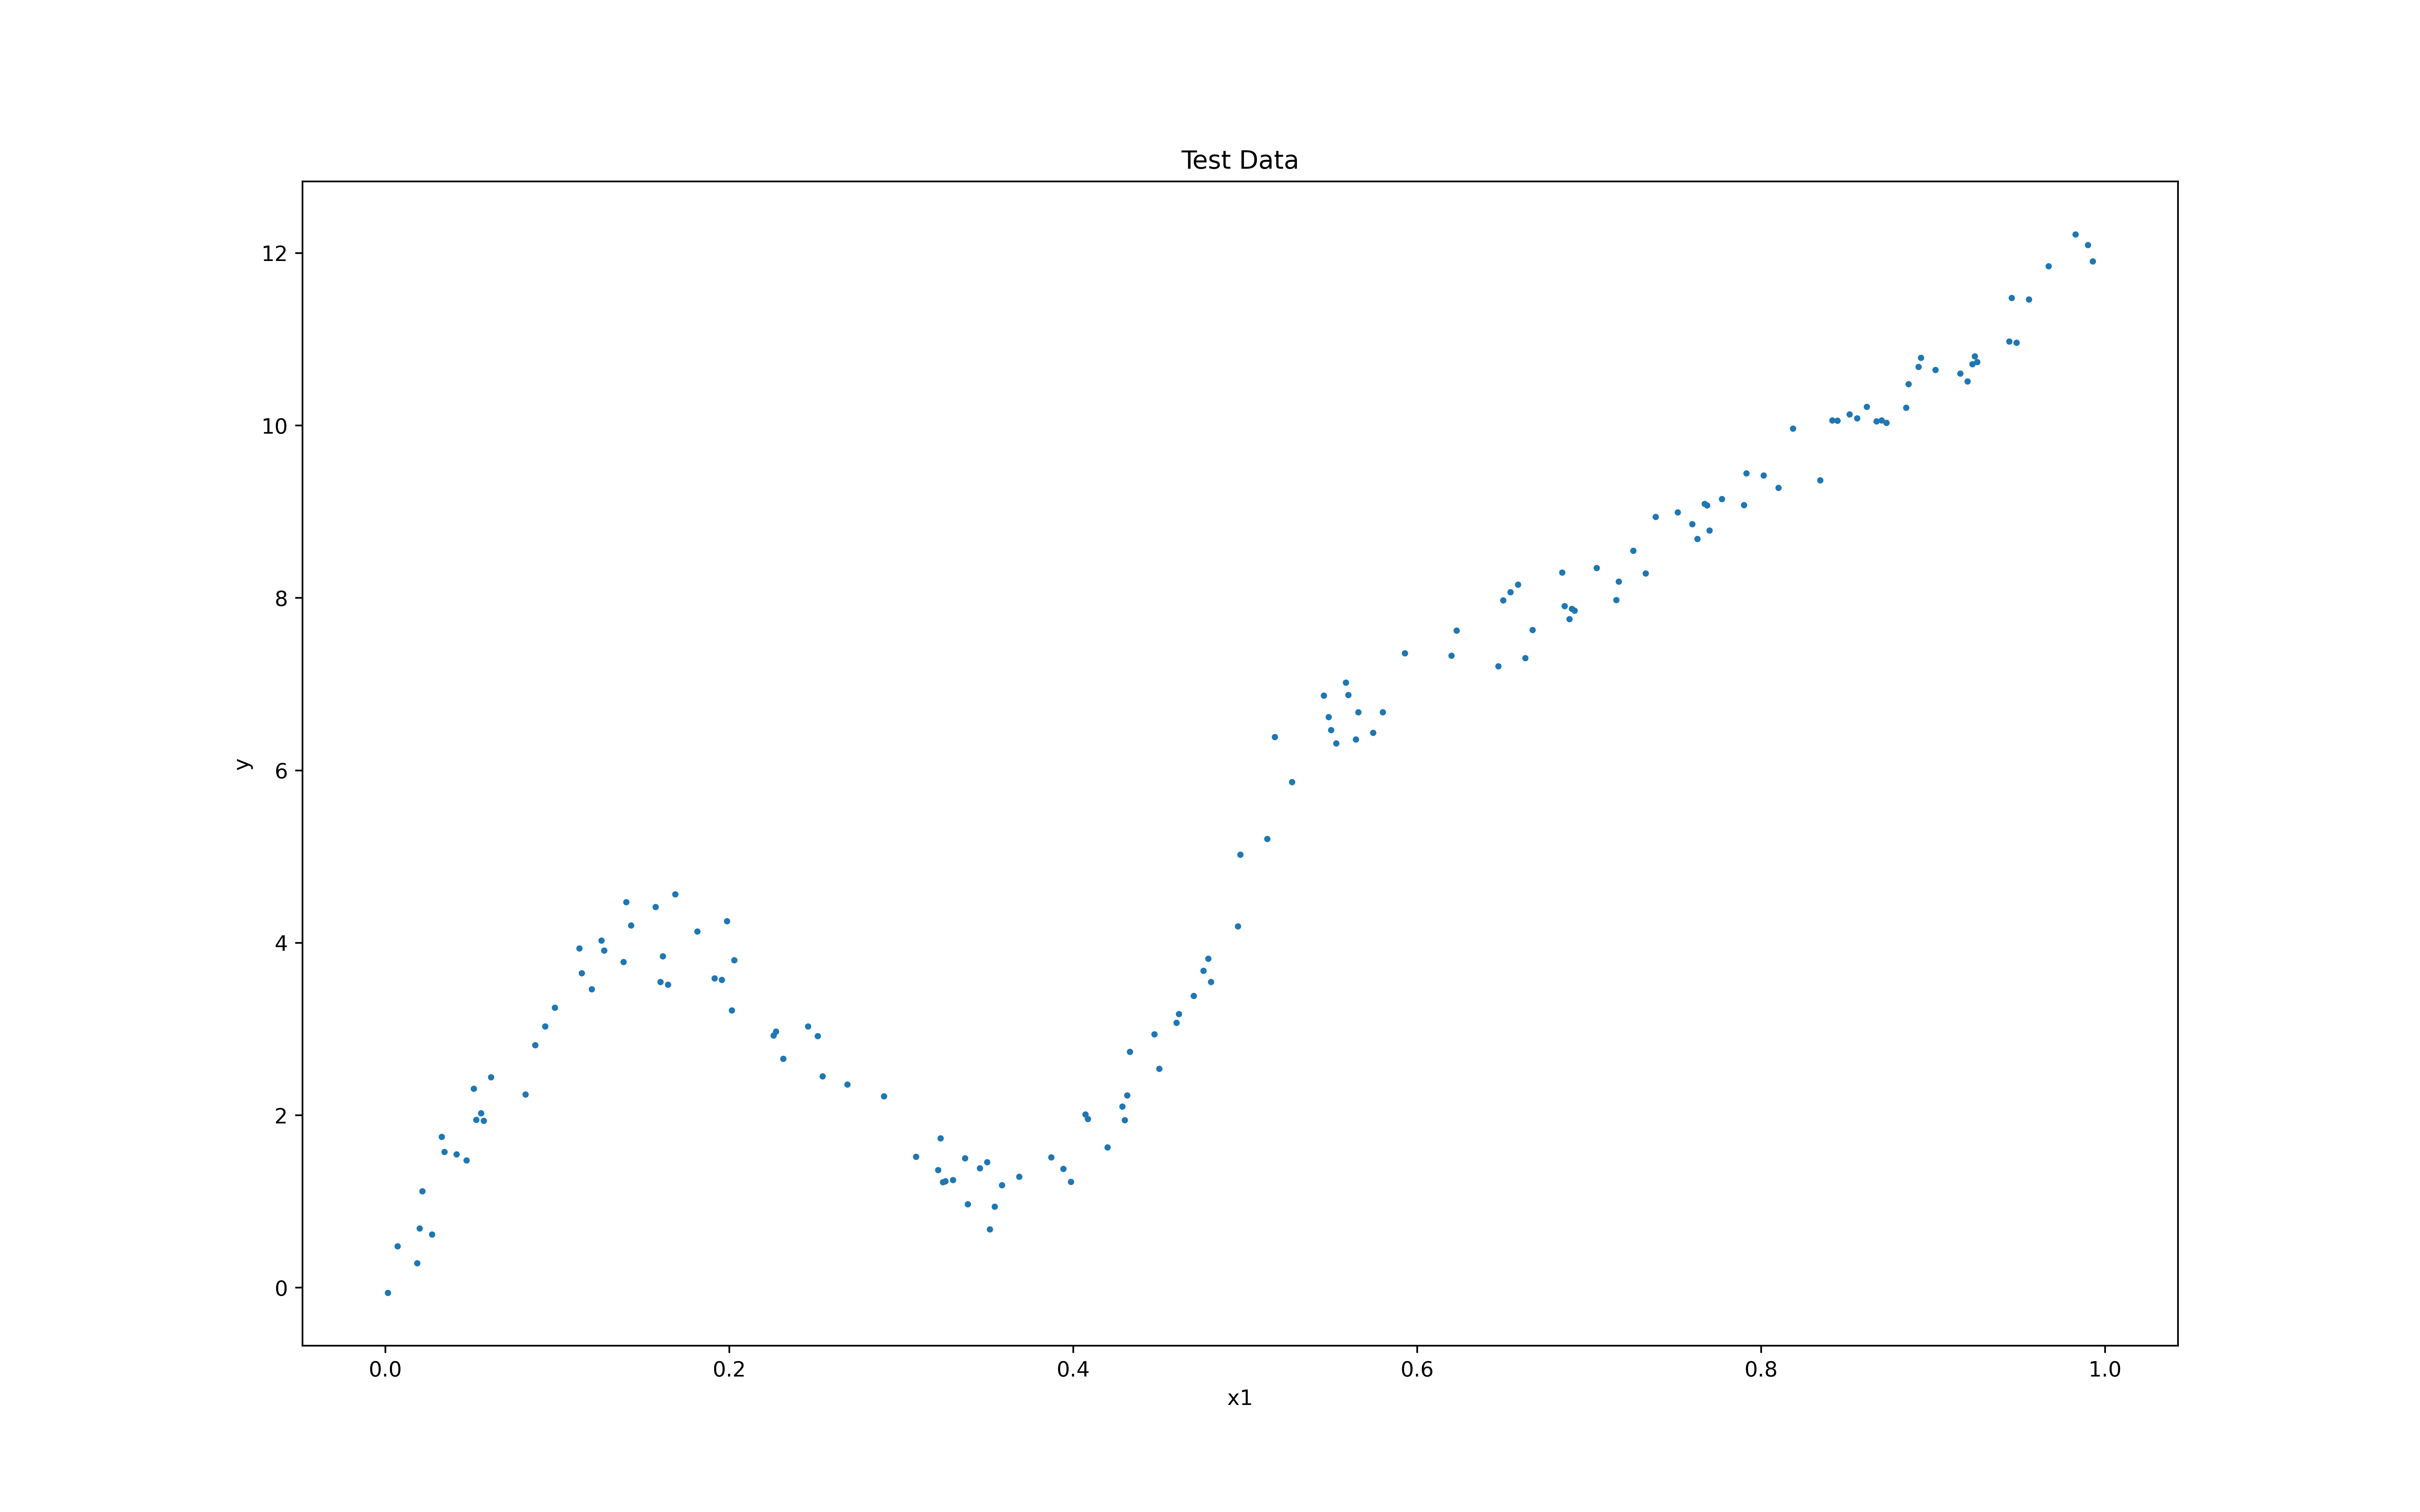
\includegraphics[width=0.7\linewidth]{./Images/E3-MLR3-Test.png}
	\caption{Testing Data used in the analysis}
\end{figure}


\clearpage